\documentclass[conference]{IEEEtran}
\usepackage{graphicx}
\usepackage{booktabs}
\usepackage{hyperref}
\graphicspath{ {images/} }
\IEEEoverridecommandlockouts

    

\begin{document}


\title{Country Image Evaluation By Aspect Based Sentiment Analysis \\
{\footnotesize \textsuperscript{}}
\thanks{}
}
 

\author{
\IEEEauthorblockN{ Karthik Puppala}
\IEEEauthorblockA{\textit{Department of Information Science} \\
\textit{University of North Texas}\\
Texas, USA \\
karthikpuppala@my.unt.edu}
\and
\IEEEauthorblockN{ Aravind Reddy Solipuram}
\IEEEauthorblockA{\textit{Department of Information Science} \\
\textit{University of North Texas }\\
Texas, USA \\
solipuramaravindreddy@my.unt.edu}
\and
\IEEEauthorblockN{  Renu Chaurasia}
\IEEEauthorblockA{\textit{Department of Information Science} \\
\textit{University of North Texas }\\
Texas, USA \\
renuchaurasia@my.unt.edu}
\and
\IEEEauthorblockN{  Abhivarma Birru}
\IEEEauthorblockA{\textit{Department of Information Science} \\
\textit{University of North Texas }\\
Texas, USA \\
abhivarmabirru@my.unt.edu}
\and
\IEEEauthorblockN{ Abhishek Puppala}
\IEEEauthorblockA{\textit{Department of Information Science} \\
\textit{University of North Texas}\\
Texas, USA \\
AbhishekPuppala@my.unt.edu}
\and
\IEEEauthorblockN{ Sreeja Suryadevara}
\IEEEauthorblockA{\textit{Department of Information Science} \\
\textit{University of North Texas}\\
Texas, USA \\
sreejasuryadevara@my.unt.edu}
}

\maketitle

\begin{abstract}

This research paper focuses on China as a representative case to examine and understand the perception of a country’s image, which holds significant influence over its inter- national relations and economic development. Utilizing an aspect- based sentiment analysis approach and a comprehensive Twitter dataset, the study aims to explore China’s image. To facilitate the analysis, Twitter dataset is manually labeled based on aspect-level sentiment annotations. Leveraging BERT which is a state- of-the-art NLP, aspect-based sentiment analysis is conducted across distinct dimensions, including Country Character, Country Competence, People Character, and People Competence. The study also investigates the perception of China’s image during the global COVID-19 outbreak, considering diverse reactions and responses from countries and populations. Understanding public sentiment toward countries is crucial in the era of social media and online communication for international relations, economic development, and tourism. The research highlights the multidimensional nature of a country’s image and emphasizes the importance of data-driven decision- making processes based on sentiment analysis. Furthermore, the research delves into the examination of China’s image during the global COVID-19 outbreak, taking into consideration the diverse reactions and responses from countries and populations. In the era of social media and online communication, understanding public sentiment towards countries is of utmost importance for international relations, economic development, and tourism. The multidimensional nature of a country’s image is highlighted, emphasizing the need for data-driven decision-making processes based on sentiment analysis.

\textbf{Index terms:}
Country Image Evaluation, Sentiment analysis, Aspect based sentiment analysis, BERT model, Topic modeling.

\textbf{Github:} \href{https://github.com/renuchaurasia/renu_INFO5731_Spring2023/tree/main/project_info5731}{Country Image Sentiment Analysis}

\end{abstract}



\section{Introduction}

A country's image and reputation are essential in shaping its international relations and economic development. A country's reputation has a big impact on how it interacts with other nations and the global community, which impacts its commerce, investment, and tourism. popular opinion is now a significant factor in determining how a nation is seen, with social media platforms like Twitter serving as an invaluable resource for real-time data on popular attitude. 

This research paper focuses on China as a representative case to explore and analyze the perception of a country's image. China's rise as a global economic and political power has generated considerable interest in understanding its image and reputation. The country's image has implications for its international trade relationships, investment attractiveness, and soft power projection. Furthermore, the global COVID-19 outbreak has highlighted the importance of a country's image, as diverse reactions and responses from countries and populations have significantly affected international relations and economic development. 

To investigate China's image, this research employs an aspect-based sentiment analysis approach. Aspect-based sentiment analysis allows for a more nuanced examination of different dimensions of a country's image, providing insights into various aspects such as Country Character, Country Competence, People Character, and People Competence. Leveraging a comprehensive Twitter dataset, the study aims to capture the real-time public sentiment towards China and analyze how it varies across different dimensions.  

The analysis in this research utilizes BERT (Bidirectional Encoder Representations from Transformers), a state-of-the-art natural language processing model known for its effectiveness in sentiment analysis. By employing BERT for aspect-based sentiment analysis, this study aims to provide a detailed understanding of the sentiment towards China's image, enabling a granular assessment of public perception. 

In addition, this research contributes to the existing body of knowledge by considering the multidimensional nature of a country's image. Previous studies have highlighted the importance of understanding multiple dimensions in evaluating a country's image. By examining different dimensions of China's image, this research aims to provide a comprehensive analysis that goes beyond simplistic binary categorizations. 

By shedding light on the perception of China's image and its impact on international relations and economic development, this research contributes to a deeper understanding of the complexities surrounding a country's reputation in the modern age. It aligns with the growing body of literature that recognizes the significance of a country's image and its implications for various aspects of national development and global interactions. 

Numerous studies have explored the relationship between a country's image and its economic outcomes. Govers and Go (2009) emphasize the role of country image in attracting foreign direct investment (FDI) and promoting export competitiveness. Similarly, Pike (2005) highlights the importance of country image in shaping tourism flows and destination choices. These studies underscore the practical implications of understanding and managing a country's image to enhance economic performance. 


In the context of China, recent research has focused on examining the country's image from various perspectives. The COVID-19 pandemic has added a new dimension to the study of a country's image. The global crisis has not only posed significant challenges to countries but also revealed how a nation's image can be affected by its handling of the situation. Kim and Kim (2020) explore the impact of COVID-19 on country image and public perceptions, emphasizing the importance of effective crisis communication and management. Shao et al. (2021) examine the role of social media in shaping public sentiment during the pandemic, demonstrating how Twitter data can be leveraged to analyze and understand the dynamics of public opinion. 
 
By utilizing an aspect-based sentiment analysis technique, this research study seeks to advance our knowledge of China's reputation by building on the body of previous work. This study gives insights into the multifaceted dimensions of China's image, including perceptions of the country's character and competence as well as the character and competence of its people, by leveraging a substantial Twitter dataset. By examining public sentiment during the global COVID-19 outbreak, this research seeks to capture the evolving dynamics of China's image and the implications for international relations, economic development, and tourism. 

\section{Related Work}

	Country Image to public perception of a particular country in areas of politics, culture ,health, economy, and diplomatic situations described by Huimin Chen, Zeyu Zhu, Fanchao Qi, Yining ye, Zhiyuan Liu, Maosong Sun, Jianbin Jin\href{https://www.ncbi.nlm.nih.gov/pmc/articles/PMC8769017/}{[1]}. Country image has a crucial impact on relations among international affairs and trade marketing. The image of a country can changes in response to global events like warfare, epidemics, and sports events. The recent pandemic, COVID-19, has had a profound impact on the image of countries. Maintaining public safety, the economy, and personal liberty during a pandemic requires governments to make decisions that can influence how their country is perceived by the international community. The actions taken by the government and the collective actions of the public can shape a country's image, which is affected by news media and framed it as a news-related issue. However, with the rise of social media platforms like Facebook, Twitter, and Reddit, it is now possible to directly investigate country image through public expressions. Researchers have started analyzing and studying the image of  China among social media through collection and analyzing tweets to understand the topics and sentiments associated with China. This has helped our project understand the definition of country image and explained about the factors and the effects of social media on computer reputation.\\

	Pappu, R., Quester, P.G. Cooksey, R.W worked on the similar topic that refers to the association’s consumers have regarding the country of origin, design, or manufacture of a product\href{https://link.springer.com/article/10.1057/palgrave.jibs.8400293#citeas}{[2]}. These associations can be at a macro level, related to the country's economic stage, or at a micro level, specific to the production of products in the country. Country image is homogenous to brand image and can be organized into meaningful groups. It can be conceptualized at the level of country and product. Macro country image encompasses all the beliefs in terms descriptive, inferential, and informational that a person perceives about any country. It includes dimensions such as economic, political, and technological aspects of the country. On the other hand, micro country image refers to the beliefs and perceptions people have towards a given country’s products. It focuses on the overall or general perception of a country's products rather than specific product categories. Some studies measure both macro and micro images to gain a comprehensive understanding. This approach overcomes the limitations of previous research that has focused promptly on either the macro or micro image of a country. This study has helped our project in understanding the effects of Country image on business and provided information about the homogeneity of Country Image and Brand equity.\\

	The Country Image dimensions has been extensively studied in marketing and behavior literature. Different variables are used to evaluate a country’s image, but the four common elements are design, prestige, innovation, and finishing. These elements pertain to the products of the country rather than the country itself. Some studies view country image as a unidimensional concept focused on product aspects, while others consider it a multidimensional concept encompassing various elements of the country. 
 
	Two common mistakes in researching country image involve failing to recognize its connection with product image and assuming it to be unchanging. The perception of a country directly affects how its products are viewed, and conversely, people's experiences with products can impact their perception of the country 
 
	Studies have proposed different dimensions for measuring the image of countries. One approach suggests three dimensions: political, economic, and technological. Another approach groups items into three categories: general attributes of country, general attributes of product, and specific attributes of the product. Another study suggests four dimensions: aspects which define the relation between products and people of the country, emotional perceptive response to the country, attitudes with arts and marketing. Importance to the global community is the fifth dimension on which a subsequent study is built upon. 

	A researcher named Ayrosa\href{https://www.researchgate.net/publication/237023445_Uma_Aplicacao_da_Abordagem_de_Personificacao_no_Estudo_de_Imagem_de_Pais
}{[3]} adapted the scale developed by Pisharodi and Parameswaran\href{https://www.acrwebsite.org/volumes/7377/volumes/v19/NA-19}{[4]}, making changes to the language, considering additional aspects, and including questions related to emotional responses. Ayrosa's work identified four dimensions: aspects related to people and products, emotional response, attitudes toward arts, and attitudes toward marketing. In a later study, Ayrosa further conducted research and refined the scale and added a fifth dimension. 

	Ayrosa’s developed scale was used in a research study involving perceptive of Dutch university students of Brazil and Brazilian products. evaluation of products, evaluation of arts, evaluation of communication and distribution, respect and importance of Brazil, and affection towards Brazil are the dimensions found in this study. These dimensions align with those identified by Ayrosa in his previous work. 
 
	Overall, the research done by Ayrosa suggests that the image of a country comprises multiple dimensions, including aspects related to products, emotional responses, arts, marketing, and global significance. These dimensions provide a more comprehensive understanding of the image of countries and can be used to assess perceptions and attitudes toward different nations. The above study has contributed in understanding the different dimension that comprises in the factors that have an impact on the image of a country. This study has helped in understanding the concept of dimensions and how a particular country has separate sets of dimensions.\\

	Sentiment analysis is a field of research that is closely connected to computational linguistics, natural language processing, and text mining.It explores effective state (psychology) and judgment (appraisal theory) using methods from data mining and computational linguistics, and it aims to answer topics that have historically been investigated in other fields of discourse.Subjectivity analysis, opinion mining, and appraisal extraction are just a few names for sentiment analysis. It also has ties to effective computing, which deals with the expression and recognition of emotion by computers. Subjective aspects, which are language representations of personal states in a certain situation, are the subject matter's main area of research.Although sentiment analysis usually believes that sentiment dwells in smaller linguistic units, these subjective elements can be single words, phrases, sentences, or even complete texts. 

	Text sentiment can be divided into two categories: explicit sentiment and implicit sentiment. Sentences that communicate an opinion in an explicit manner are referred to as explicit sentiment. An example would be, "It's a beautiful day." On the other hand, implicit sentiment suggests an opinion, like in the statement "The earphone broke in two days." Since explicit sentiment is thought to be simpler to evaluate, most current work in sentiment analysis focuses exclusively on doing so. 

	Text analysis considers sentiment polarity. Although polarity is frequently split into positive and negative categories, it can also be thought of as a range rather than a binary classification. A document including a variety of opinionated remarks would not be entirely impartial; instead, it would have a mixed polarity overall. The difference between the polarity and the strength of a sentiment must also be made. Due to a lack of experience, one may feel strongly that a thing is merely okay, neither exceptionally good nor poor, or weakly that it is excellent.  

	Finding the target of sentiment, which can be a thing, a concept, a person, or anything else, is an important part of sentiment analysis. Since it is very simple to identify the topic in product and movie reviews, a large portion of earlier research in the field concentrated on analyzing sentiment in those evaluations. It is useful to know which exact characteristics of the subject are being discussed, though. For instance, it's crucial to say whether a product review is criticizing the camera display or the battery life. In the past ten years, there has been a great deal of research done on extracting these attributes from language, both in explicit remarks (such as "Battery life is too short") and implicit references (such as "Camera is too large").

	This work has contributed in understanding the base concept of sentiment analysis. It gave us the understanding of the principles of sentiment analysis and the field of works which contributed in better understanding of sentiment analysis.\\
	
	Sentiment analysis is a task in natural language processing that involves evaluating the sentiment orientation of a text. It seeks to identify sentiment polarity and extract views from unstructured text \href{https://www.sciencedirect.com/science/article/abs/pii/S0950705118306105}{[5]}. Aspect-based sentiment analysis (ABSA) is a branch of sentiment analysis that focuses on locating the characteristics or aspects \href{https://www.sciencedirect.com/science/article/abs/pii/S0925231219311920}{[6]} of the target entities and the sentiments expressed toward each one. Due of its proficiency in gleaning valuable information from reviews and user comments, ABSA has grown in popularity. 
	
	However, challenges continue to exist with current ABSA methods. Finding the precise linking of aspect terms and opinion words can be difficult since, without domain expertise, the semantic relationship between the components in a phrase may not be obvious. Additionally, while existing ABSA methodologies work effectively, they frequently don't provide justifications for the classification of a given aspect-sentiment information as positive or negative. There is a need for an explainable strategy that makes use of domain knowledge to deal with these problems \href{https://www.sciencedirect.com/science/article/abs/pii/S0925231219311920}{[7]}. In studies on cognition and human-level intelligence, knowledge graphs\href{https://www.sciencedirect.com/science/article/abs/pii/S0893608019301613}{[8]}, which depict the structural links between items, have gained popularity. A sentiment knowledge graph (SKG) is a collection of trustworthy sentiment data that has been manually selected. Given that it reveals the underlying connections between aspect keywords and sentiment words in texts, it can be a useful tool for aspect-sentiment information identification. The efficiency of sentiment analysis may be increased by using an SKG, and classifications of aspects of sentiment can be explained.\\
	
	By using an SKG to capture high-order aspect-sentiment interactions, the authors of this work offer a unique method for explainable aspect-based sentiment analysis. They offer a sentiment analysis approach known as the knowledge-enabled BERT model, which expands on the K-BERT\href{https://www.sciencedirect.com/science/article/abs/pii/S0167739X20309195}{[9]} language representation paradigm. The system generates contextualized representations using BERT\href{https://www.sciencedirect.com/science/article/abs/pii/S0957417422021467}{[10]}, a well-known pre-trained language model with Transformer. Furthermore, the sentiment knowledge network is incorporated as an external source of sentiment domain information, improving sentiment detection performance by introducing domain knowledge into BERT. This project has benefited from this work's grasp of the fundamental ideas of aspect-based sentiment analysis and the significance of aspects. This work has helped in the analysis of the many features. This graph has helped with learning about knowledge graphs.\\
	

	The increasing trend of people living more of their lives online, especially on social media and e-commerce platforms. This shift has been accelerated by the COVID-19 pandemic and the need for social distancing. Understanding the emotional content generated on online platforms such as Yelp and delivery platforms can provide business insights and personalized recommendations. Sentiment analysis techniques have been applied to analyze the emotional content on micro blogs, online reviews, narratives, and other social media. 

	User-generated reviews contain complex information beyond overall sentiment. Aspect-Based Sentiment Analysis (ABSA) focuses on identifying different aspects embedded within a text and their associated sentiment. Targeted ABSA (TABSA) is a more general version that considers multiple targets in a review, each with their associated aspects. Neural models, including deep neural networks and self-attention models like BERT, have been used for ABSA and TABSA with promising performance improvements. However, these models often treat BERT as a black box and don't fully leverage the contextual information. 

	The study about Targeted ASBA and BERT approach\href{https://arxiv.org/pdf/2010.07523.pdf}{[11]} aims to improve the BERT model architecture to be context-aware. The authors introduce two methods: Context-Guided BERT (CG-BERT) and Quasi-Attention Context-Guided BERT (QACG-BERT). CG-BERT adapts a context-aware self-attention network for ABSA, while QACG-BERT introduces quasi-attention weights and subtractive attention. The contributions of the approach include extending the context-aware self-attention network to ABSA, achieving state-of-the-art results on ABSA datasets with QACG-BERT, and analyzing how context influences the self-attention and decisions of the models.
	
\section{Data Collection}

We are using the data collected from twitter and news social media. For the above collected data, we have manually labeled the four aspects, such as Country Competence. Six variables in the dataset correspond to:

\begin{enumerate}

\item \textbf{Text:} text values of tweet data 

\item \textbf{Sentiment: } discrete value based on the sentiment of text.

\item \textbf{Country Competence:} discrete value based on the sentiment of the managing and addressing the country related issues.

\item \textbf{Country Character:} discrete value based on the sentiment of the identity and political character.

\item \textbf{People Competence:} discrete value based on the sentiment of the people education and creativity.

\item \textbf{People Character:} discrete value based on the sentiment of the trust and integrity of the population.

\end{enumerate}

\begin{figure}[h]
\centering
 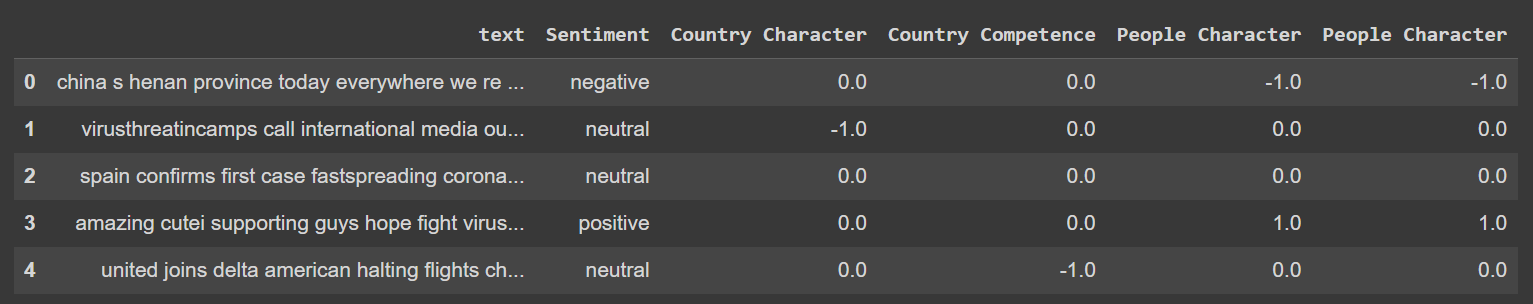
\includegraphics[width=9cm]{dataset}
 \caption{dataset of twitter}
 \end{figure}
 
\begin{figure}[h]
\centering
 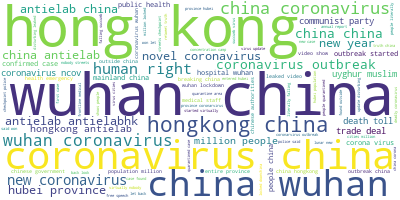
\includegraphics[width=9cm]{WordCloud}
 \caption{Dataset WordCloud}
 \end{figure}

The dataset is pre processed with following various steps:

\begin{enumerate}

\item \textbf{Filtering and removing irrelevant data:}
Twitter data often contains noise and irrelevant information such as URLs, hashtags, mentions, and special characters. During this step, you would filter out or remove these elements to focus on the actual text content. For example, you can remove URLs using regular expressions or filter out tweets that are purely retweets or contain specific keywords that indicate irrelevance.


\item \textbf{Converting non-uniform data into a standard format:}
Twitter data is usually informal and may contain various forms of abbreviations, misspellings, emoticons, and non-standard punctuation. Converting non-uniform data into a standard format involves tasks such as correcting misspellings, expanding abbreviations, and normalizing punctuation. For example, converting "u" to "you" or replacing "gr8" with "great" would help standardize the text.


\item \textbf{NLTK using a "Stop Word Dictionary":}
The Natural Language Toolkit (NLTK) is a popular library for NLP tasks in Python. Stop words are commonly used words in a language (e.g., "and," "the," "is") that do not carry significant meaning and can be safely ignored. NLTK provides a stop word dictionary that contains a predefined list of such words. During preprocessing, you would remove these stop words from the text data to reduce noise and focus on more meaningful words and phrases.


\item \textbf{Lemmatization/stemming:}
Lemmatization and stemming are techniques used to transform words to their root form. Lemmatization considers the context and meaning of words and transforms them to their base or dictionary form (known as lemmas). Stemming, on the other hand, applies simpler rules to strip word suffixes to obtain the word stem. For example, both lemmatization and stemming would transform "running" to "run" or "cats" to "cat." The goal is to reduce the dimensionality of the data and consolidate different word forms into their common root form.

\end{enumerate}

\section{The methodology }

 
The section describes a data-driven generated coding investigation framework for analyzing sentiments related to different aspects of a country and its people. It illustrates our framework integrating the Raw Twitter Data to predict the sentiment of people about the China Image from Fig-1. The analysis procedure encompasses four stages: 
\begin{enumerate}
\item parsing the raw Twitter data, performing data cleaning and preprocessing.
\item manually constructing an aspect-level sentiment dataset.
\item forecasting the sentiment for each aspect \item analyzing the gathered sentiments.\\
\end{enumerate}

\begin{figure}[h]
\centering
 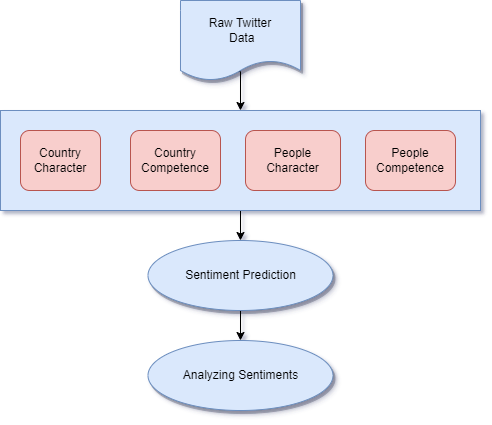
\includegraphics[width=9cm]{FlowChart}
 \caption{Framework of Country Image Evaluation}
 \end{figure}
 
\begin{figure}[h]
\centering
 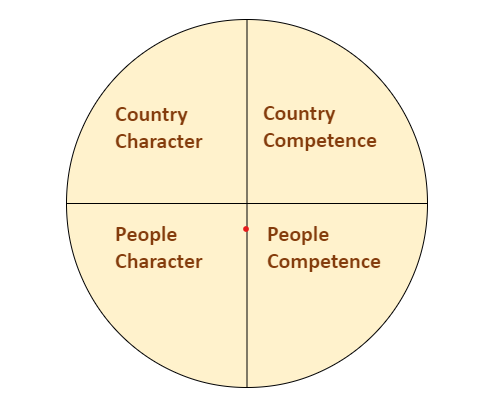
\includegraphics[width=9cm]{PieChartAspects}
 \caption{Framework of Aspects based sentiments}
 \end{figure}

The Aspect level of sentiment consists of four categories: 


 \textbf{Country Character:} refers to how effectively one understands a country's identity and political character. This means that the sentiment analysis will be based on how people perceive the country's image, reputation, and political values. For example, people may view a country as democratic, authoritarian, or corrupt, and this will affect their sentiment towards the country.
 
 \textbf{Country Competence:} refers to how effectively the country manages and addresses the issues related to economy and social policies or cultural and technological competence. This means that the sentiment analysis will be based on how people perceive the country's ability to manage economic and social policies, or its competence in areas such as culture and technology. For example, people may view a country as innovative, prosperous, or unstable, and this will affect their sentiment towards the country.
 
 \textbf{People Competence:} refers to how people view the health, education, and creativity of the population. This means that the sentiment analysis will be based on how people perceive the level of education, health care, and creativity of the country's population. For example, people may view a country as having a highly educated and healthy population, or as lacking in these areas, and this will affect their sentiment towards the country.
 
 \textbf{People Character:} refers to how people view the hard work, trust, and integrity of the population. This means that the sentiment analysis will be based on how people perceive the values and behavior of the country's population. For example, people may view a country as having a hardworking and trustworthy population, or as being corrupt and untrustworthy, and this will affect their sentiment towards the country.\\
 
\begin{table}[]
\centering
\caption{Aspect based sentiments}
\label{tab:my-table}
\resizebox{\columnwidth}{!}{%
\begin{tabular}{c|c|c|c|}
\cline{2-4}
                                     & \textbf{Positive} & \textbf{Negative} & \textbf{Neutral} \\ \hline
\multicolumn{1}{|c|}{\textbf{Country Character}} & 20           & 77            & 100             \\ \hline
\multicolumn{1}{|c|}{\textbf{Country Competence}}  & 20          & 60           & 120         \\ \hline
\multicolumn{1}{|c|}{\textbf{People Character}}   & 19        & 40          & 130         \\ \hline
\multicolumn{1}{|c|}{\textbf{People Competence}}   & 20            & 30          & 130               \\ \hline
\end{tabular}%
}\\
\end{table}

\textbf{Topic Modeling}

Topic modeling is a statistical approach that utilizes unsupervised machine learning techniques to identify clusters or groups of related words within a given text corpus. Unlike traditional methods, topic modeling does not rely on predefined tags or training data but instead extracts semantic structures from the text itself.

By analyzing the content of documents, topic modeling aims to uncover common themes or topics and organize them into meaningful clusters. For instance, it can determine if incoming documents belong to categories such as contracts, invoices, complaints, or others based on their textual characteristics.

Latent Dirichlet Analysis (LDA) is widely recognized as a prominent technique in topic modeling. By examining the connections among words within a document, LDA reveals the underlying structure within a collection of observations. In LDA, documents are viewed as a combination of topics, and topics are viewed as a combination of words. When analyzing multiple documents, LDA assumes that they share similar topics but with distinct distributions.\\


\textbf{BERT Model}

BERT (Bidirectional Encoder Representations from Transformers) is a state-of-the-art natural language processing (NLP) model developed by Google researchers. It is a deep learning model based on the Transformer architecture that has revolutionized various NLP tasks.  

BERT’s key technical innovation is applying the bidirectional training of Transformer, a popular attention model, to language modeling. This is in contrast to previous efforts which looked at a text sequence either from left to right or combined left-to-right and right-to-left training. 

BERT makes use of a Transformer, an attention mechanism that learns contextual relations between words (or sub-words) in a text. In its vanilla form, Transformer includes two separate mechanisms — an encoder that reads the text input and a decoder that produces a prediction for the task. 

BERT relies on a Transformer (the attention mechanism that learns contextual relationships between words in a text). Bidirectional Encoder Representations from Transformers, is a language representation model that has achieved state-of-the-art results in many natural language processing tasks. BERT is based on the Transformer architecture, which consists of an encoder and a decoder. However, since BERT's goal is to generate a language representation model, it only utilizes the encoder portion of the Transformer. The input to BERT's encoder consists of a sequence of tokens, which are first converted into vectors and then processed by the neural network. To enhance the input, BERT also utilizes three types of embeddings: token embeddings, segment embeddings, and positional embeddings.


BERT needs the input to be massaged and decorated with some extra metadata:
    
\begin{enumerate}

\item \textbf{Token embeddings}: involve adding special tokens such as [CLS] at the beginning of the first sentence and [SEP] at the end of each sentence. These tokens serve as markers for the start and end of each sentence and allow BERT to handle multiple sentences in a single input.
    
\item \textbf{Segment embeddings}: are used to distinguish between different sentences. A marker indicating whether a token belongs to the first sentence or the second sentence is added to each token.
    
\item \textbf{Positional embeddings}: are added to each token to indicate its position in the sentence. Since the order of the tokens is important for understanding the meaning of the sentence, positional embeddings allow BERT to encode the sequence information of the input.
\end{enumerate}

 \begin{figure}[h]
\centering
 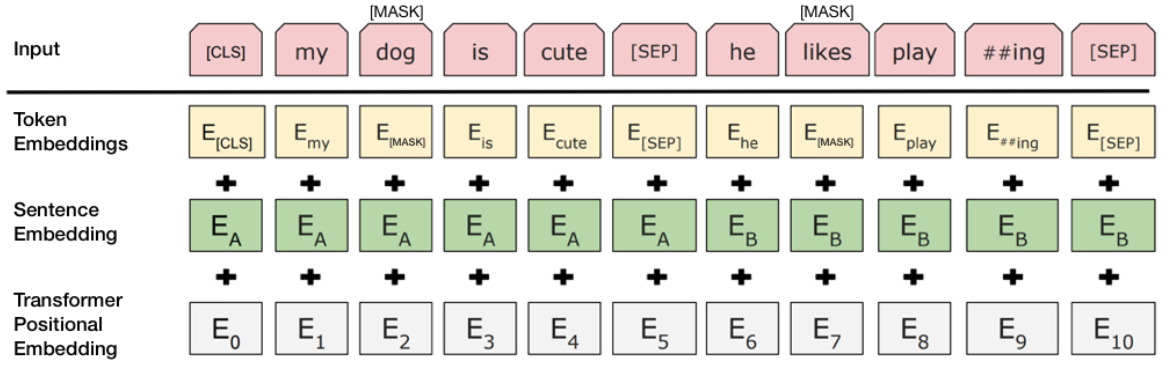
\includegraphics[width=9cm]{BERT}
 \caption{ BERT [Devlin et al., 2018], with modifications}
 \end{figure}
 
	The Transformer architecture employs a sequence-to-sequence mapping, where each layer processes sequences and produces corresponding output sequences. Consequently, the output of the Transformer is also a sequence of vectors, maintaining a one-to-one correspondence between the input and output tokens at corresponding indices. It is worth noting that BERT, unlike some other models, does not attempt to predict the subsequent word in a sentence.\\

	In the BERT (Bidirectional Encoder Representations from Transformers) model, input IDs and attention masks play crucial roles in the input encoding process. Input IDs are essentially a sequence of integers that represent the tokens present in the input text. These tokens are assigned their respective token IDs from the model's vocabulary. By converting the input text into a series of token IDs, BERT ensures that the model understands and processes the text in a standardized format. This representation allows BERT to effectively capture the semantic meaning of the tokens and learn contextual relationships between them.\\

	The attention mask is a sequence of 0s and 1s that serves as a guiding mechanism for the model's attention mechanism. It indicates which tokens in the input sequence should receive attention from the model and which ones should be ignored. By setting the attention mask to 1 for relevant tokens and 0 for padding tokens, BERT can selectively attend to important parts of the input sequence while disregarding irrelevant or padded tokens. This is particularly useful when dealing with variable-length input sequences, where padding is necessary to create uniform-length input batches. By attending to relevant tokens and ignoring padding tokens, the attention mask helps BERT focus on the essential information in the input sequence, improving the model's ability to understand and make predictions based on the input.\\

	By using the attention mask, the BERT model benefits from improved performance and enhanced contextual understanding. The attention mechanism allows the model to weigh the importance of different tokens in the input sequence based on their relevance to the task at hand. By assigning higher attention weights to meaningful tokens and lower weights to padding tokens, BERT can effectively allocate its processing resources to the most informative parts of the input. This selective attention enables the model to better capture the semantic relationships between tokens and understand the context in which they appear. Consequently, the attention mask helps BERT optimize its predictions and achieve higher accuracy in various natural language processing tasks, such as text classification, named entity recognition, and question-answering.\\
	
\begin{figure}[h]
\centering
 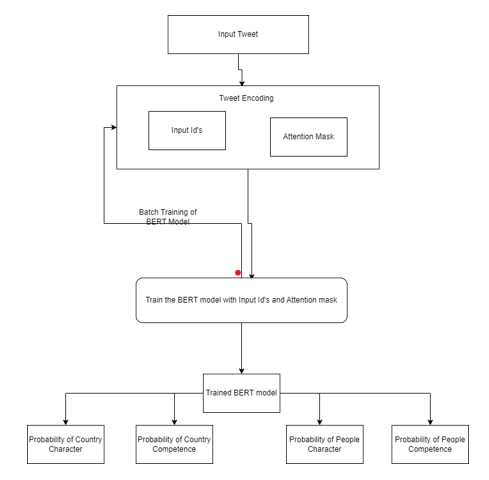
\includegraphics[width=9cm]{BERT_Flow}
 \caption{Model Architecture}
 \end{figure}

\section{The results}
 
The overall attitude seen in the early COVID-19 pandemic stages. On social media sites like Twitter, there was a lot of fear, confusion, and disinformation floating about at the time, which contributed to a generally unpleasant mood in public conversation. It is not unexpected to see that your dataset follows this pattern and that more unfavourable opinions are stated for each feature.

Our research project provided analysis of China's reputation, using a combination of sentiment analysis and topic modelling techniques. Our findings suggest that while China's reputation is viewed more negatively than positively.

\begin{figure}[h]
\centering
 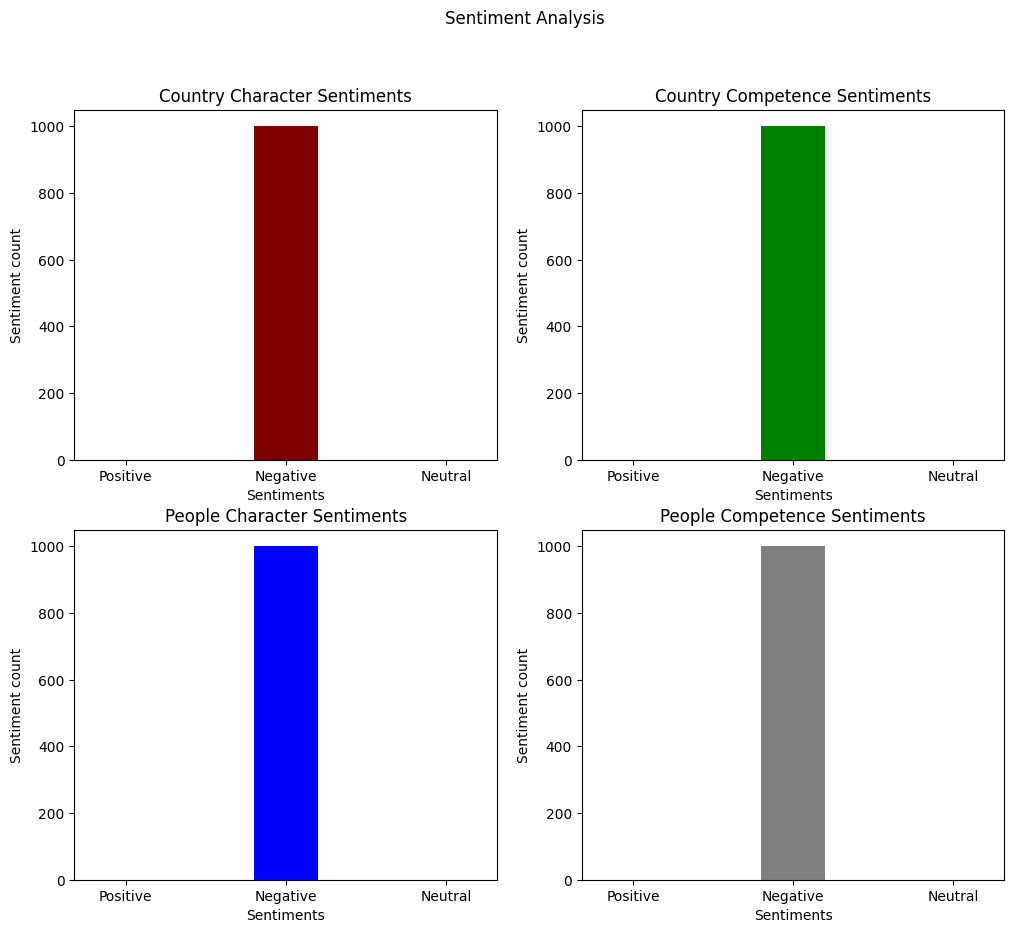
\includegraphics[width=9cm]{results}
 \caption{Aspect based sentiment prediction results}
 \end{figure}

Additionally, it could be intriguing to go more deeply into the particular elements that were examined and discover any underlying causes for the unfavorable opinion. For instance, if one of the characteristics included government acts or policies, it could be worthwhile to investigate how the general public felt about them and whether any particular instances contributed to a more unfavorable perception
 

\section{Conclusion and Limitations}

 This research aimed to evaluate the impact of the COVID-19 pandemic on China's reputation through an analysis of public opinion on Twitter. Through sentiment analysis and natural language processing techniques, we found that China's reputation on Twitter was viewed more negatively than positively, with sentiment scores falling into the negative category for most aspects. Our analysis also revealed that the most common topics mentioned in relation to China's reputation were economic development, international relations, human rights, and cultural heritage. These findings suggest that China's reputation has been impacted by the pandemic, as well as ongoing issues in these areas.

Overall, this research provides insights into how global crises can impact a country's reputation and highlights the importance of understanding public sentiment on social media platforms. The results can be valuable for policymakers, businesses, and other organizations that have an interest in understanding China's global reputation and how it may impact their operations. Additionally, this research can inform efforts to improve China's reputation in the international community in the aftermath of the pandemic.

\section{Author Contributions}

\begin{enumerate}

\item \textbf{Aravind Reddy Solipuram:} worked on implementation of the bert model with training data and following the different techniques and scenarios and performed topic modeling.
\item \textbf{Karthik Puppala:} worked on implementation of the bert model with training data and following the different techniques and scenarios and performed topic modeling.
\item \textbf{Renu Chaurasia:} Data Cleaning of the huge dataset by removing the unnecessary columns and contributed to creating dataset with only required columns consisting of twitter data and performed Data Pre-processing by removing the null values, missing values and has documented the project.
\item \textbf{Abhivarma Birru:} Data Cleaning and  Data Pre-processing. Cleaning of data by removing null values, missing values, and unwanted data. Performed preprocessing by removing the stop words and contributed to creating dataset with only required columns consisting of twitter data and Performed the Data Visualization of the initial data.
\item \textbf{Abhishek Puppala:} Data Pre-processing by employing lemmatization, removing punctuations, symbols and emojis of twitter data. and Performed the Data Visualization of the initial data, test data and predicted Data.

\end{enumerate}


\begin{thebibliography}{00}
	\bibitem{b1} Chen, H., Zhu, Z., Qi, F., Ye, Y., Liu, Z., Sun, M.,  Jin, J. (2020). Country image in COVID-19 pandemic: A case study of China. IEEE Transactions on Big Data, 7(1), 81-92. 
	\bibitem{b2} Z. Yang, H. Men and R. Ingham, "Media Representation of China in COVID-19 Reports: Text Mining of the Language of New York Times," 2022 European Conference on Natural Language Processing and Information Retrieval (ECNLPIR), Hangzhou, China, 2022, pp. 101-107, doi: 10.1109/ECNLPIR57021.2022.00030. 
	\bibitem{b3} Vaswani, A., Shazeer, N., Parmar, N., Uszkoreit, J., Jones, L., Gomez, A. N., ...  Polosukhin, I. (2017). Attention is all you need. Advances in neural information processing systems, 30. 
	\bibitem{b4}de Moura Engracia Giraldi, J., Ikeda, A. A.,  Campomar, M. C. (2011). Reasons for country image evaluation: A study on China image from a Brazilian perspective. Journal of Database Marketing  Customer Strategy Management, 18, 97-107. 
	\bibitem{b5} Kumar, V. (2022). Spatiotemporal sentiment variation analysis of geotagged COVID-19 tweets from India using a hybrid deep learning model. Scientific Reports, 12(1), 1849. 
	\bibitem{b6} Tang, S.,  Willnat, L. (2023). News exposure and Americans’ perceptions of China in 2019 and 2021. Online Media and Global Communication, 2(1), 54-76. 
	\bibitem{b7} Zhao, X., You, X.,  Lin, S. (2022). China's country image in the eyes of international students from central Asian countries. Frontiers in Psychology, 13. 
	\bibitem{b8} 
	\bibitem{b9} R. Mohan Pisharodi and Ravi Parameswaran (1992) ,"Confirmatory Factor Analysis of a Country-Of-Origin Scale: Initial Results", in NA - Advances in Consumer Research Volume 19, eds. John F. Sherry, Jr. and Brian Sternthal, Provo, UT : Association for Consumer Research, Pages: 706-714. 
	\bibitem{b10} A. Chinnalagu and A. K. Durairaj, "Comparative Analysis of BERT-base Transformers and Deep Learning Sentiment Prediction Models," 2022 11th International Conference on System Modeling  Advancement in Research Trends (SMART), Moradabad, India, 2022, pp. 874-879, doi: 10.1109/SMART55829.2022.10047651.
	\bibitem{b11} A. J. Nair, V. G and A. Vinayak, "Comparative study of Twitter Sentiment On COVID - 19 Tweets," 2021 5th International Conference on Computing Methodologies and Communication (ICCMC), Erode, India, 2021, pp. 1773-1778, doi: 10.1109/ICCMC51019.2021.9418320. 
	\bibitem{b12} Y. Zhao, E. Soerjodjojo and H. Che, "Methods to Enhance BERT in Aspect-Based Sentiment Classification," 2022 Euro-Asia Conference on Frontiers of Computer Science and Information Technology (FCSIT), Beijing, China, 2022, pp. 21-27, doi: 10.1109/FCSIT57414.2022.00016. 
	\bibitem{b13} M. T. Riaz, M. Shah Jahan, S. G. Khawaja, A. Shaukat and J. Zeb, "TM-BERT: A Twitter Modified BERT for Sentiment Analysis on Covid-19 Vaccination Tweets," 2022 2nd International Conference on Digital Futures and Transformative Technologies (ICoDT2), Rawalpindi, Pakistan, 2022, pp. 1-6, doi: 10.1109/ICoDT255437.2022.9787395. 
	\bibitem{b14} N. T. M. Trang and M. Shcherbakov, "Vietnamese Question Answering System f rom Multilingual BERT Models to Monolingual BERT Model," 2020 9th International Conference System Modeling and Advancement in Research Trends (SMART), Moradabad, India, 2020, pp. 201-206, doi: 10.1109/SMART50582.2020.9337155. 
	\bibitem{b15} Pappu, R., Quester, P. G., Cooksey, R. W. (2007). Country image and consumer-based brand equity: relationships and implications for international marketing. Journal of International Business Studies, 38, 726-745.
	\bibitem{b16} Pisharodi, R. M., Parameswaran, R. (1992). Confirmatory factor analysis of a country-of-origin scale: initial results. ACR North American Advances.
	\bibitem{b17} Liu, F., Cohn, T., Baldwin, T. (2018). Recurrent entity networks with delayed memory update for targeted aspect-based sentiment analysis. arXiv preprint arXiv:1804.11019.
	\bibitem{b18} Yang, M., Jiang, Q., Shen, Y., Wu, Q., Zhao, Z., Zhou, W. (2019). Hierarchical human-like strategy for aspect-level sentiment classification with sentiment linguistic knowledge and reinforcement learning. Neural Networks, 117, 240-248.
	\bibitem{b19} Saeidi, M., Bouchard, G., Liakata, M., Riedel, S. (2016). Sentihood: Targeted aspect based sentiment analysis dataset for urban neighbourhoods. arXiv preprint arXiv:1610.03771.
	\bibitem{b20} Punetha, N., Jain, G. (2023). Bayesian game model based unsupervised sentiment analysis of product reviews. Expert Systems with Applications, 214, 119128.
	\bibitem{b21} Elbagir, S., Yang, J. (2019, March). Twitter sentiment analysis using natural language toolkit and VADER sentiment. In Proceedings of the international multiconference of engineers and computer scientists (Vol. 122, p. 16).
	\bibitem{b22} Sethia, K., Saxena, M., Goyal, M., Yadav, R. K. (2022, April). Framework for Topic Modeling using BERT, LDA and K-Means. In 2022 2nd International Conference on Advance Computing and Innovative Technologies in Engineering (ICACITE) (pp. 2204-2208). IEEE.
	\bibitem{b23} Manurung, R. (2008). Machine learning-based sentiment analysis of automatic indonesian translations of english movie reviews. In Proceedings of the International Conference on Advanced Computational Intelligence and Its Applications (ICACIA) (pp. 1-6).
	\bibitem{b24} Buntoro, G. A., Adji, T. B., Purnamasari, A. E. (2016). Sentiment Analysis Candidates of Indonesian Presiden 2014 with Five Class Attribute. International Journal of Computer Applications, 975(136.2), 23-29.
	\bibitem{b25} Soelistio, Y. E., Surendra, M. R. S. (2015). Simple text mining for sentiment analysis of political figure using naive bayes classifier method. arXiv preprint arXiv:1508.05163.
	\bibitem{b26} Kim, J., Ko, Y., Kim, W., Kim, G., Lee, J., Eyman, O. T. G., ... Lee, W. K. (2023). Understanding the Impact of the COVID-19 Pandemic on the Perception and Use of Urban Green Spaces in Korea. International Journal of Environmental Research and Public Health, 20(4), 3018.
	\bibitem{b27}Hoang, M., Bihorac, O. A., Rouces, J. (2019). Aspect-based sentiment analysis using bert. In Proceedings of the 22nd nordic conference on computational linguistics (pp. 187-196).
	\bibitem{b28}Chiorrini, A., Diamantini, C., Mircoli, A., Potena, D. (2021, March). Emotion and sentiment analysis of tweets using BERT. In EDBT/ICDT Workshops (Vol. 3).
	\bibitem{b29} Xu, H., Liu, B., Shu, L., Yu, P. S. (2019). BERT post-training for review reading comprehension and aspect-based sentiment analysis. arXiv preprint arXiv:1904.02232.
	\bibitem{b30}Geetha, M. P., Renuka, D. K. (2021). Improving the performance of aspect based sentiment analysis using fine-tuned Bert Base Uncased model. International Journal of Intelligent Networks, 2, 64-69.
\end{thebibliography}



\end{document}